\documentclass[10pt]{article}
\usepackage{fullpage}

\usepackage{epsf}
\usepackage{graphicx}
\graphicspath{{.}{./graphics/}{../graphics/}}

%\pagestyle{empty}
\begin{document}

\newcommand{\richard}{{Richard T.~Vaughan}}
\newcommand{\kasper}{{Kasper St{\o}y}}
\newcommand{\gaurav}{{Gaurav S.~Sukhatme}}
\newcommand{\maja}{{Maja J.~Matari\'{c}}}
\newcommand{\brian}{{Brian P.~Gerkey}}
\newcommand{\andrew}{{Andrew Howard}}

\begin{center}
{\Large Agents 2001 Demonstration Proposal\\
\vspace*{.5em}
Player \& Stage : Distributed Device Control \& Simulation}\\
\vspace*{2em}
\brian, \richard, \andrew, \gaurav~\& \maja\\
USC Robotics Research Labs\\
Los Angeles, CA\\
\end{center}

\section*{Summary}
The University of Southern California Robotics Research Lab has a
significant program of research into intelligent agents. We evaluate
our systems and techniques using a variety of robots, sensors and
simulation models.

To facilitate this work we have developed infrastructure software that
that will be of interest and use to other students and researchers:
Player and Stage.  Player is a device server that provides a simple
abstract interface to a number of different physical sensing and
actuation devices. Stage provides a population of simulated Player
devices with an identical external interface.

Player has quickly become the most-used interface to all the devices
in our labs. It is an essential part of our program to exploit
distributed sensing, control and communication in multi-agent systems
by abstracting away the details of each device and giving transparent
network access to any device at any time. It is also a very convenient
platform for more conventional robot experiments.

This kind of infrastructure is a prerequisite to implementing any
multi-agent control system, and we believe that together, Player and
Stage could become a standard on which such systems are built, saving
development time by code re-use, and encouraging comparative
evaluation. We believe Player and Stage will be immediately useful to
the Autonomous Agents community, and we aim to develop them into a
commodity product.  Source for both programs is freely available under
the GPL; see {\tt
  http://robotics.usc.edu/\hspace{.05cm}${}_{\tilde{}}$\hspace{.05cm}player}
for source code and documentation.


\section*{The Software}
{\bf Player} is a distributed multi-threaded device server.  It provides a
software interface to all of the sensors and actuators that we use in
our lab.  Device drivers within Player allow it to abstract away
device particulars, such as message protocols, data formats, and
timing, making it suitable for use by students with little programming
experience. Yet the researcher still has full access to and control of
the device if required. Player currently supports the devices that
make up the popular ActivMedia Pioneer 2 mobile research robot (wheel
motors, odometry, sonar, compass, etc.), and many peripherals such as
a scanning laser rangefinder, pan-tilt-zoom cameras, frame grabbers
and sound hardware, which we use both on our robots and in other,
standalone, embedded sensing situations.  Also, we employ ``virtual''
devices, which do not map precisely to physical hardware, but rather
do some processing or aggregation of data and/or commands.  For
example, as an aid in robot localization, we have developed a {\sl
  beacon-detector} device that performs intelligent signal processing
on laser range data to identify specially constructed beacons in the
environment.  These extra devices become part of Player itself,
providing a mechanism for sharing and reusing work within our lab (and
around the world) in much the same way as Linux kernel modules are
used.

Player provides a unified network socket interface to its devices, allowing
clients to be written in virtually any programming language on 
any computing platform.  We currently provide interface libraries
(to handle messaging details) in C, C++, Java, and Tcl/Tk, with
others, such as Python and Matlab, in the works.  Further, the
network-level abstraction allows a client program to execute
anywhere that has connectivity to the Player server.
This ability, combined with Player's integral support for multiple
clients' concurrent access to devices enables the construction
of arbitrarily sophisticated distributed multi-agent control
systems.

Player has an elegant modular design which makes adding new devices
very easy. We encourage researchers to add device drivers to our
repository to create a library that supports many common pieces of
hardware, and provides many useful virtual devices.

\noindent {\bf Stage} simulates a user-defined population of Player devices, allowing
development and testing of agent architectures and controllers in an
environment very similar to that provided by the real hardware. Stage
spawns several copies of Player, replacing the real device drivers
with its simulated equivalents. The user interfaces with Player in the
normal way; clients see the identical interface to real and simulated
hardware. As in Player, devices are implemented as modules and can be
easily added or modified by a moderately experienced programmer.

Stage provides a graphical user interface to the world and its
devices, allowing the experimenter to easily manipulate devices (e.g.
moving robots around in the world; panning camera devices, etc.).
Stage also provides a logging mechanism that is independent of Player
for ground-truthing.

We have found that agents developed in simulation will work with
little or no modification on the real devices and vice-versa. The
Stage distribution includes a variety of environments suitable for
large and small-scale experiments in multi-agent sensing,
communications and control.

In its default configuration, Stage simulates (0$<$N$<$254) mobile
robots moving in and sensing a two-dimensional bitmapped environment,
controlled through Player.  Various sensor models are provided,
including sonar, scanning laser rangefinder, a pan-tilt-zoom camera,
color blob tracking and odometry.  Stage provides good enough fidelity
to transfer controllers designed in simulation to the real robots, yet
it is efficient enough to simulate large populations. Our aim is to
provide a simulated version of every Player device as far as possible.


\section*{Description of Demonstration}
We will demonstrate the use of Player and Stage in a variety of
configurations.  Specifically, we will show networks in which multiple
clients and multiple robots are connected in different ways to form
useful multi-agent systems.  We will show some of the tools we have
developed for Player and Stage, such as graphical displays and data
loggers.  These demonstrations will be carried out both in simulation
and with a Pioneer 2 mobile robot equipped with a variety of
peripheral devices.  To showcase the fact that Stage's external
interface is identical to that of Player, we plan to map the
demonstration area, construct an equivalent environment in the
simulator, and demonstrate the same client program controlling both
physical and simulated robots.

We will display posters describing the Player architecture,
implementation and suggested applications, and invite feedback from
the delegates to help us improve the software. 

\section*{Requirements}

We can run the demo in two different modes; a live software demo with
video presentation of the robot and sensor hardware; or if funds
permit, we can bring robots to give a more compelling demonstration.
In either case we will need poster space, a large monitor or projector
for our laptop screen and a table. For robots we would need some open
space in which our robot will roam around. An internet connection
would be very useful.  We would be powering/charging several things,
such as robots, laptops, and batteries, so we may need as many as 10
110VAC/60Hz power outlets.

We propose to run the demo with two students, or one student and a
postdoc, and request assistance with travel and registration costs. If
the live robot/sensor demo is preferred, we would also need to insure
some equipment (the expensive laser scanner, camera \& robots).

\section*{Contact}

Brian Gerkey or Richard Vaughan [gerkey,vaughan]@robotics.usc.edu. 

\noindent Phone: 213 740 4523\\
Fax: 213 740 7512


\begin{figure}
\begin{center}
\includegraphics[width=100mm]{pioneer_ants}
\caption{\label{fig:pioneers}Four Pioneer 2 robots with SICK LMS-200 laser rangefinders; these robots run the Player server to provide network-transparent access to all their sensors and actuators. .}
\end{center}
\end{figure}


\begin{figure}
 \centering
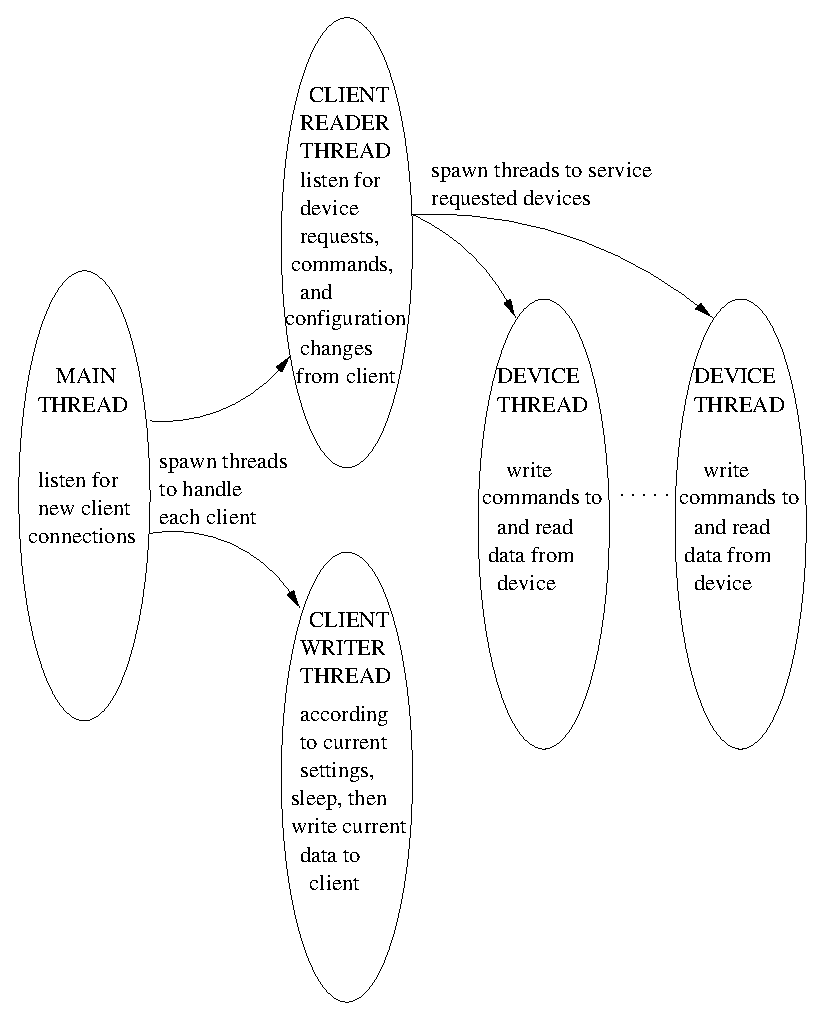
\includegraphics[width=100mm]{threads}
  \caption{{\sl Dynamic thread hierarchy of Player}}
\label{figure:threads}
 \end{figure} 

\begin{figure}
 \centering
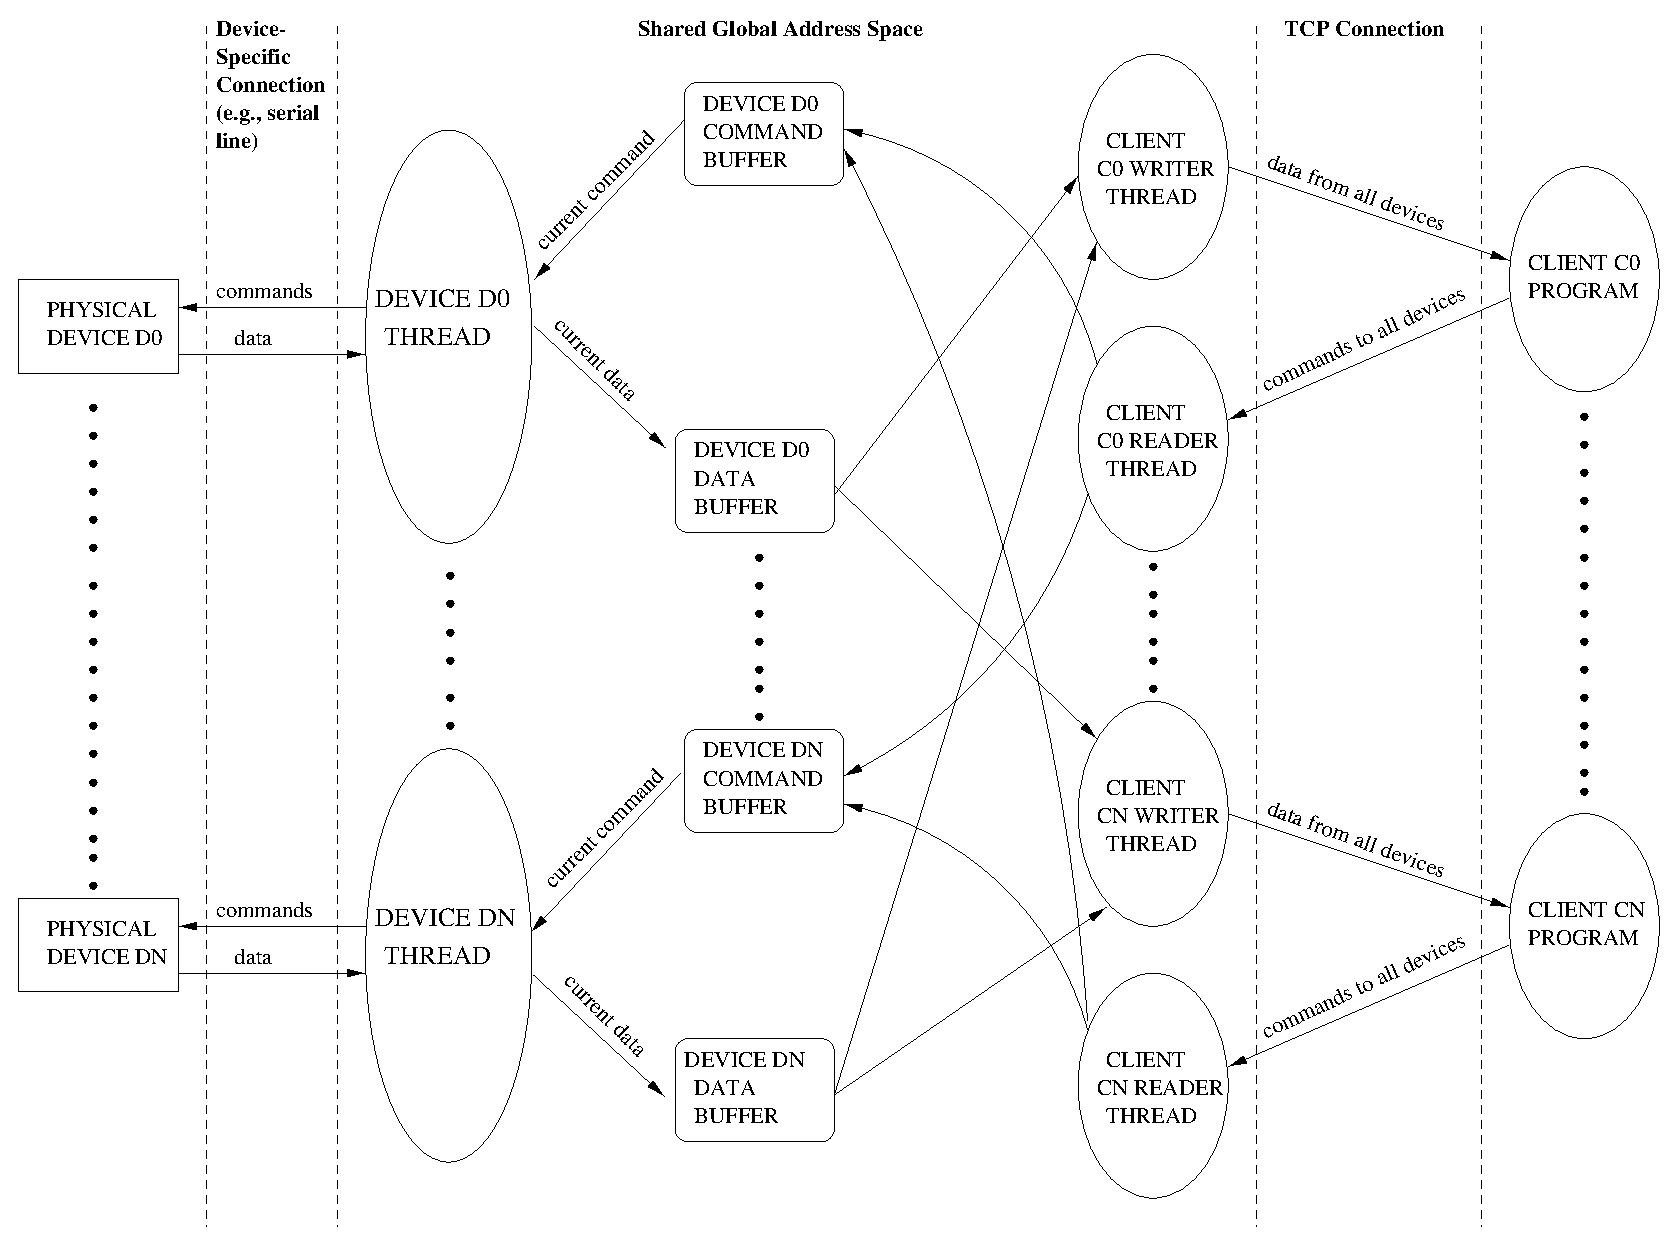
\includegraphics[width=100mm]{buffers}
  \caption{{\sl Overall system architecture of Player}}
  \label{figure:buffers}
\end{figure} 

 \begin{figure}
    \begin{center}
      \includegraphics[width=100mm]{stage_hospital_grey}
 \caption{\label{fig:hospital}Screenshot from Stage showing 12 robots moving 
   in one of the example environments (hospital.world). The bitmap was
   imported from a CAD model of a real hospital building; it is
   approximately 6 times the width and 4 times the height of the area
   shown. Stage enables agent experiments in large, complex
   environments with populations of sensors, robots and communications
   devices that may not be available in the real world. }
\end{center}
\end{figure}


\begin{figure}
\begin{center}
\includegraphics[width=100mm]{device_visualization_grey}
\caption{\label{fig:devicedetails}Screenshot of Stage showing the rendering of detailed device information for a robot using sonar and PTZ camera (toggled with the middle mouse button). }
\end{center}
\end{figure}


\begin{figure}
\begin{center}
\includegraphics[width=150mm]{stage_structure}
\caption{\label{fig:iostructure}Stage system diagram, showing the I/O relationships between processes and threads in a running Stage system.}
\end{center}
\end{figure}


\end{document}
